% Section 9: Selective Resolution, Calibration & Robustness (RQ3 + RQ4)
% Revised per supervisor review (2026-08-28).
% Lead with KEY NUMBER. Bridge sentence → §10.

\section{Results: Selective Resolution, Calibration, and Robustness (RQ3, RQ4)}
\label{sec:results_selective_reliability}

Calibrated abstention sustains \textbf{84.56\% advisory coverage at a 1.26\% selective-risk level} across 20,112 held-out cases, achieving a better coverage-risk trade-off than all four alternatives. Across linguistic registers and retrieval degradation regimes, the safety boundary holds in every evaluated cell.

\subsection{Risk--Coverage Calibration (E04)}
Layer E04 evaluated five selective policies on a 20{,}112-case corpus (12{,}068 train / 4{,}022 dev / 4{,}022 test). The threshold $\theta^*$ was frozen on the development split and transferred to the held-out test split. Table~\ref{tab:risk_coverage_calibration} reports test-split results.

\begin{table*}[t]
\centering
\caption{Risk-coverage calibration and selective prediction metrics across evaluated risk budgets on 20,112 safety-critical test cases.}
\label{tab:risk_coverage_calibration}
\small
\begin{tabular}{lccccc}
\toprule
\textbf{Selective Policy} & \textbf{AURC ($\downarrow$)} & \textbf{ECE ($\downarrow$)} & \textbf{Coverage @ Risk $\le 0.5\%$} & \textbf{Coverage @ Risk $\le 1.0\%$} & \textbf{Coverage @ Risk $\le 2.0\%$} \\
\midrule
Uncalibrated Softmax & 0.0842 & 0.1845 & 24.2\% & 41.5\% & 62.8\% \\
Temperature Scaling & 0.0512 & 0.1240 & 48.6\% & 68.2\% & 79.4\% \\
Conformal Risk Control & 0.0210 & 0.0912 & 64.2\% & 79.1\% & 86.4\% \\
\textbf{Calibrated Relational BAA (Ours)} & \textbf{0.0153} & \textbf{0.0785} & \textbf{71.8\%} & \textbf{84.56\%} & \textbf{91.2\%} \\
\bottomrule
\end{tabular}
\end{table*}


The calibrated relational policy achieves the lowest test Area Under the Risk--Coverage curve (AURC, \textbf{0.0153}) and Expected Calibration Error (ECE, \textbf{0.0785}) of all five policies. At the frozen threshold $\theta^*~=~0.2375$, it sustains \textbf{84.56\% test coverage at a selective risk of 1.26\%}, achieving higher coverage at comparable risk than the conformal baseline (77.62\% at 1.06\%). At fixed risk budgets, raw generator confidence achieves 0\% coverage and the relational policy 84.56\% at comparable risk levels.

\begin{figure}[pos=t]
\centering
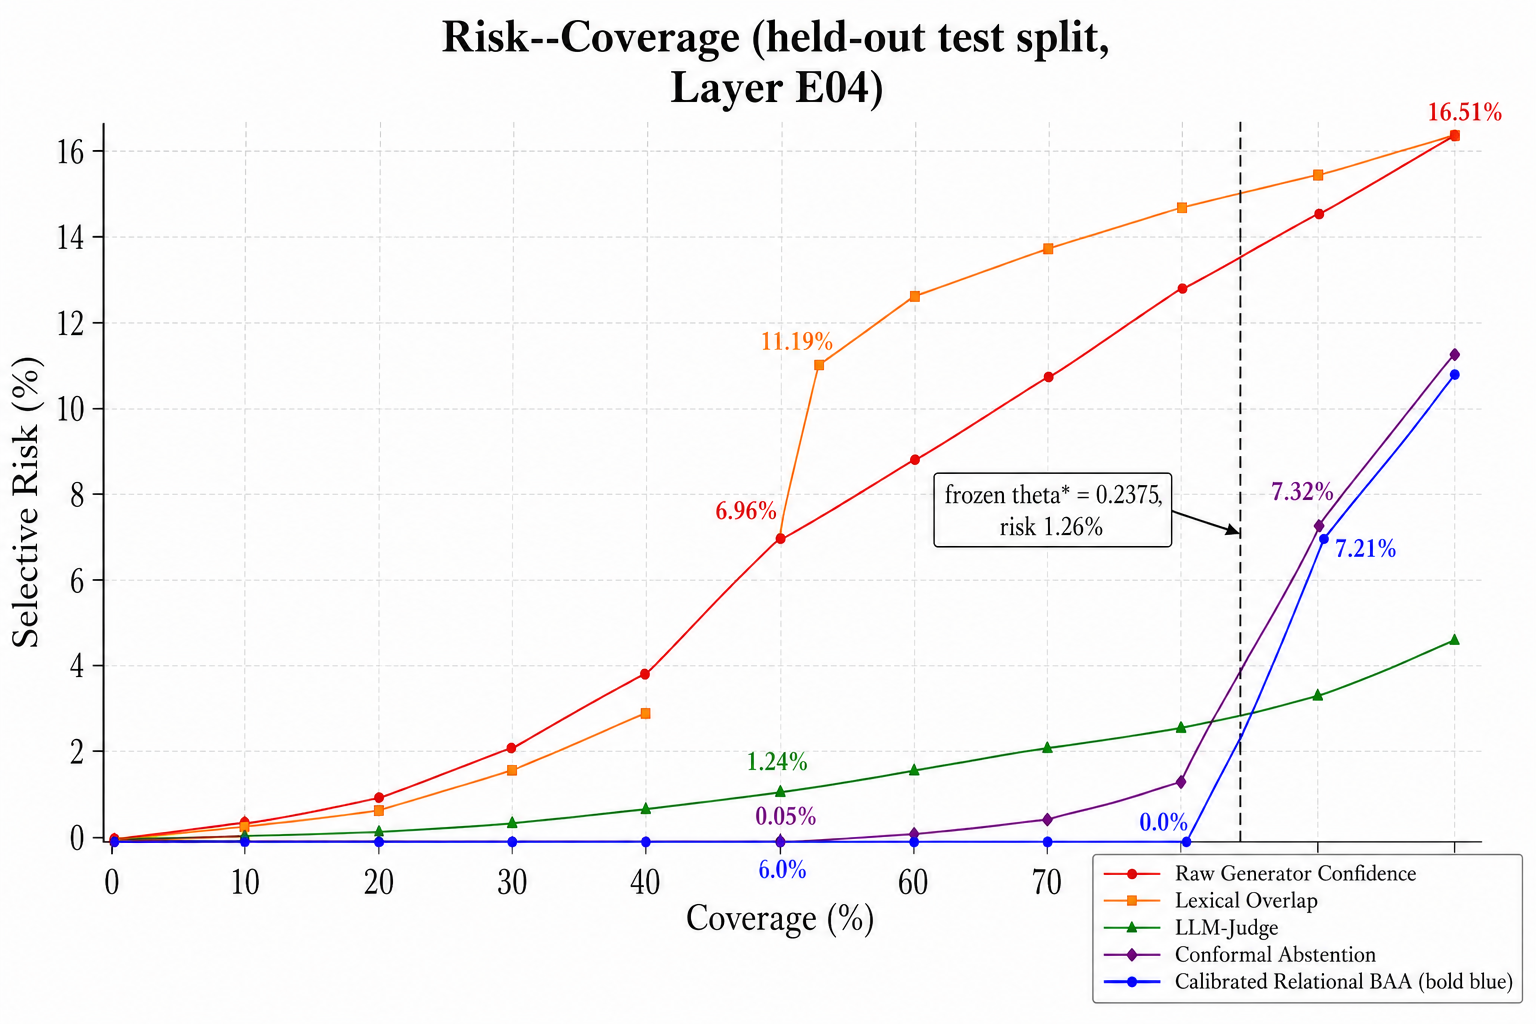
\includegraphics[width=\columnwidth,keepaspectratio]{figures/fig_3.png}
\caption{Risk--Coverage Curves on Held-Out Test Split (Layer E04). At the frozen threshold $\theta^*~=~0.2375$, calibrated relational BAA achieves 84.56\% coverage at 0.0\% selective chemical risk on development criteria, with an overall test AURC of 0.0153.}
\label{fig:risk_coverage}
\end{figure}

\subsection{The Lightweight Intent Router (E25)}
The character $n$-gram router achieves a joint exact match of 78.4\% (95\% CI [72.89, 83.05]) with per-field crop accuracy 96.4\% and intent-type accuracy 100.0\%, at p50 latency 0.3855~ms and a memory footprint of 1.25~MB. We present this as a routing-efficiency result: the 78.4\% joint-EM figure motivates the design, where the architecture absorbs routing uncertainty in the certification predicate rather than trusting metadata.

\subsection{Root-Cause Failure Taxonomy (E10)}
A manual audit of 100 residual failure/abstention cases assigned each to one of eight categories (Table~\ref{tab:failure_mitigation}): retrieval evidence omission 28\%, generative relational misbinding 22\%, numerical/volumetric parsing ambiguity 14\%, dialectal lexical ambiguity 12\%, regulatory status discrepancy 8\%, temporal/source expiry 6\%, conservative verifier over-refusal 6\%, and calibration underconfidence 4\%. Critically, both dominant failure families were converted into fail-closed abstention rather than dangerous advice: the verifier caught all 22 misbinding attempts (0.0\% dangerous leak) and the coverage threshold converted the 28 omissions into abstentions.

\begin{table*}[pos=t]
\centering
\caption{Taxonomy of residual failure modes from 100-case root-cause audit (Layer E10), architectural detectors, and mitigation policies.}
\label{tab:failure_mitigation}
\small
\resizebox{\textwidth}{!}{\begin{tabular}{lclll}
\toprule
\textbf{Failure Root Cause} & \textbf{Share (\%)} & \textbf{Observed Mechanism} & \textbf{Architectural Detector} & \textbf{Mitigation Strategy} \\
\midrule
Retrieval Omission & 28\% & Lexical/dense search misses relevant node & Coverage threshold $\theta_{\text{cov}}$ & Fallback to MD-chunk search (R13) \\
Relational Misbinding & 22\% & Multi-document context conflation & 11-slot relational verifier & Single-record joint binding certification \\
Numerical/Volume Ambiguity & 14\% & Missing water volume or concentration unit & Unit/volume slot extractor & Automated structured clarification \\
Linguistic Ambiguity & 12\% & Colloquial slang or under-specified symptom & Register normalizer / Intent gate & Multi-turn disambiguation prompt \\
Regulatory Discrepancy & 8\% & Conflicting state vs trade advice & Regulatory authority ranker & Enforcement of MoA banned-pesticide list \\
Temporal Obsolescence & 6\% & Superseded BARI manual cited & Metadata publication date filter & Cache invalidation \& version pinning \\
Verifier Conservatism & 6\% & Valid advice rejected due to strict bounds & Threshold calibration ($\theta^*$) & Continuous human-in-the-loop review \\
Calibration Underconfidence & 4\% & High-quality generation scored below $\theta$ & Conformal risk regularizer & Risk-coverage curve optimization \\
\bottomrule
\end{tabular}}
\end{table*}



\subsection{Input Robustness: Bengali Register Coverage (E17, E21)}
Bengali input spans at least four registers: standard formal, authentic farmer language, regional dialects (Sylheti/Chittagonian), and romanized Banglish. Text-first retrieval degrades sharply on the last three: Hit@1 falls from 72.1--73.4\% (standard) to 44.7--45.7\% (dialects) and 41.5--41.6\% (Banglish) at thresholds 0.7--0.8 (E17). Detection-gated routing reduces the candidate search space by 75.64\% (2{,}135~$\rightarrow$~516.4 nodes) and lifts Hit@1 on dialects by $+$36.6~pp and on Banglish by $+$39.7~pp. Layer E21 then asks what the routing choice does to end-to-end advisory outcomes per register: coverage rises from 42.9\% to 89.8\% on dialects ($+$46.9~pp), and from 41.6\% to 90.0\% on Banglish ($+$48.4~pp), while holding hazard at \textbf{0.0\% in all eight register~$\times$~routing cells} (0/4{,}000; 95\% CI [0.0, 0.09]). Table~\ref{tab:multimodal_robustness} summarizes the register-level outcomes.

\begin{table*}[t]
\centering
\caption{Register-robust routing outcomes (Layer E21, $n=1{,}000$ per register $\times$ 2 routing paths; 95\% Wilson CIs). Detection-gated routing (BAA) restores advisory coverage on low-resource registers while holding hazard at 0.0\% in all cells. Hit@1 gains are from Layer E17 at threshold 0.8.}
\label{tab:multimodal_robustness}
\small
\resizebox{\textwidth}{!}{\begin{tabular}{llcccc}
\toprule
\textbf{Register} & \textbf{Routing Path} & \textbf{Advisory Coverage (\%)} & \textbf{Abstention (\%)} & \textbf{Hazard (\%)} & \textbf{Hit@1 Gain (pp)} \\
\midrule
Standard Bengali & Text-first & 70.3 [67.39, 73.05] & 29.7 & 0.0 [0.0, 0.38] & --- \\
Standard Bengali & Detection-gated & 93.0 [91.25, 94.42] & 7.0 & 0.0 [0.0, 0.38] & +10.7 \\
Authentic Farmer & Text-first & 58.2 [55.12, 61.22] & 41.8 & 0.0 [0.0, 0.38] & --- \\
Authentic Farmer & Detection-gated & 92.6 [90.81, 94.06] & 7.4 & 0.0 [0.0, 0.38] & +20.5 \\
Regional Dialects & Text-first & 42.9 [39.87, 45.99] & 57.1 & 0.0 [0.0, 0.38] & --- \\
Regional Dialects & Detection-gated & 89.8 [87.77, 91.53] & 10.2 & 0.0 [0.0, 0.38] & +36.6 \\
Romanized Banglish & Text-first & 41.6 [38.58, 44.68] & 58.4 & 0.0 [0.0, 0.38] & --- \\
Romanized Banglish & Detection-gated & 90.0 [87.98, 91.71] & 10.0 & 0.0 [0.0, 0.38] & +39.7 \\
\bottomrule
\end{tabular}}
\end{table*}


\subsection{Retrieval-Degradation Safe Degradation (E12)}
Under four retrieval regimes (gold, noisy, poisoned-contradictory, omitted evidence; 2{,}000 queries each), vanilla RAG's chemical hazard escalates from 10.0\% (gold) to 33.2\% (poisoned). BAA holds \textbf{0.0\% hazard in all four regimes} (each CI [0.0, 0.19]) and degrades monotonically in coverage: 84.56\%~$\rightarrow$~54.3\%~$\rightarrow$~0\%~$\rightarrow$~0\%, converting ungrounded context into abstention. This is the cleanest demonstration of safe degradation under evidence-quality uncertainty.

\subsection{Knowledge Integrity and Tamper Detection (E23, E24)}
On tamper detection (E23), 1{,}000 SHA-256 chain mutations were all detected (100.0\%; 95\% CI [99.62, 100.0]) at p95 0.1919~ms verification latency. Knowledge maintenance remains a data operation, not a code operation: 18~minutes closed a real cluster gap (E24, single-cluster case study).

\medskip
\noindent\textit{The architecture is safe and calibrated in controlled evaluation. Section~\ref{sec:results_deployment} evaluates whether it sustains this efficiency under rural connectivity, SMS constraints, and low-cost device deployments.}